\subsection{Tredicesimo sprint}

\begin{minipage}{\textwidth}
  Di seguito è riportata la distribuzione delle ore per ciascun membro del team, accumulate in totali per persona e per ruolo:
  \begin{table}[H]
    \begin{tabularx}{\textwidth}{|c|*{6}{>{\centering}X|}c|}
      \hline
      \multicolumn{8}{|c|}{\textbf{Consuntivo orario}} \\
      \hline
      \textbf{Membro del team} & \textbf{Re} & \textbf{Am} & \textbf{An} & \textbf{Pt} & \textbf{Pr} & \textbf{Ve} & \textbf{Totale per persona} \\
      \hline
      Riccardo Cavalli & 0 & 0 & 1 & 2 & 4 & 1 & 8 \\
      \hline
      Raul Pianon & 1 & 0 & 1 & 0 & 4 & 1 & 7 \\
      \hline
      Martina Dall'Amico & 1 & 0 & 1 & 2 & 4 & 2 & 10 \\
      \hline
      Marco Cristo & 0 & 1 & 0 & 4 & 3 & 2 & 10 \\
      \hline
      Sebastiano Lewental & 1 & 0 & 1 & 2 & 4 & 2 & 10 \\
      \hline
      Mattia Zecchinato & 0 & 1 & 0 & 4 & 3 & 2 & 10 \\
      \hline
      Tommaso Stocco & 1 & 0 & 1 & 5 & 3 & 1 & 11 \\
      \hline
      \textbf{Totale ore per ruolo} & 4 & 2 & 5 & 19 & 25 & 11 & \textbf{66} \\
      \hline
    \end{tabularx}
    \caption{Sprint 13 - Consuntivo orario}
  \end{table}
  \end{minipage}

  \begin{figure}[H]
    \centering
    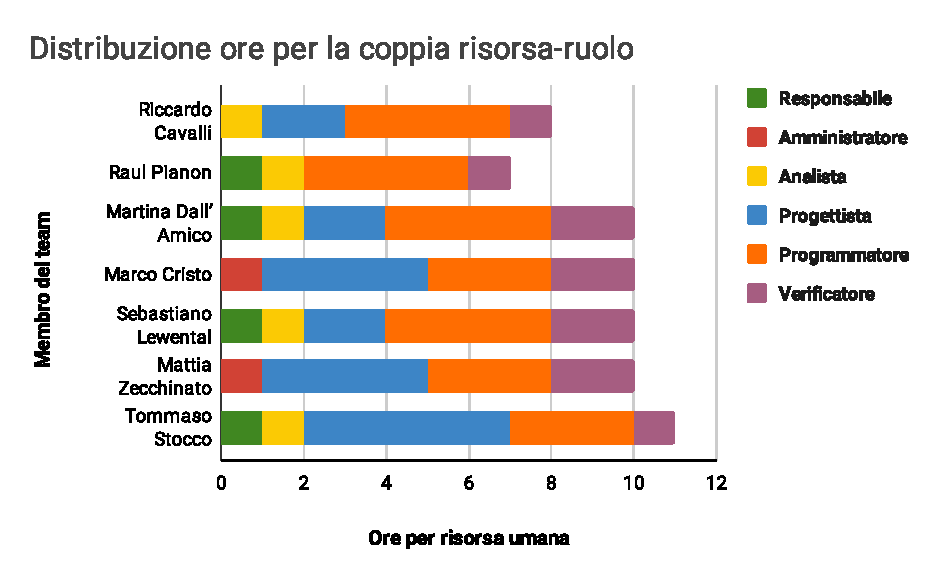
\includegraphics[width=0.90\textwidth]{assets/Consuntivo/Sprint-13/distribuzione_ore_risorsa_ruolo.pdf}
    \caption{Sprint 13 - Istogramma della distribuzione oraria per la coppia risorsa-ruolo}
  \end{figure}

  \begin{figure}[H]
    \centering
    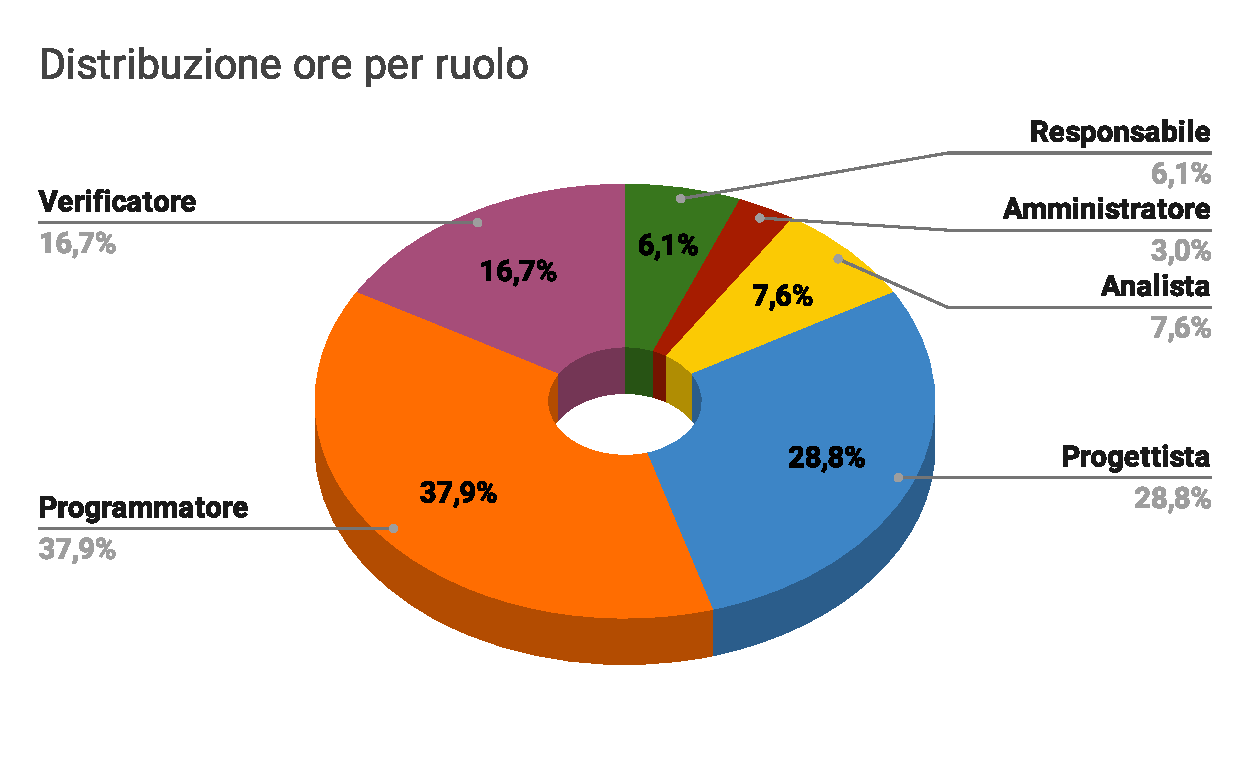
\includegraphics[width=0.90\textwidth]{assets/Consuntivo/Sprint-13/distribuzione_ore_ruolo.pdf}
    \caption{Sprint 13 - Areogramma della distribuzione oraria per ruolo}
  \end{figure}

  \begin{minipage}{\textwidth}
  Di seguito è riportato il consuntivo economico del tredicesimo \glossario{sprint}:
  \begin{table}[H]
  \begin{adjustwidth}{-0.5cm}{-0.5cm}
    \centering
    \begin{tabular}{|P{2.9cm}|P{2.3cm}|P{2.5cm}|P{2.3cm}|>{\arraybackslash}P{2.5cm}|}
      \hline
      \multicolumn{5}{|c|}{\textbf{Consuntivo economico}} \\
      \hline
      \textbf{Ruolo} & \textbf{Ore per ruolo} & \textbf{Delta ore preventivo - consuntivo} & \textbf{Costo (in \texteuro)} & \textbf{Delta costo preventivo - consuntivo (in \texteuro)} \\
      \hline
      \Responsabile[U]{} & 4 & 0 & 120,00 & 0,00 \\ \hline
      \Amministratore[U]{} & 2 & 1 & 40,00 & 20,00 \\ \hline
      \Analista[U]{} & 5 & 0 & 125,00 & 0,00 \\ \hline
      \Progettista[U]{} & 19 & 0 & 475,00 & 0,00 \\ \hline
      \Programmatore[U]{} & 25 & 0 & 375,00 & 0,00 \\ \hline
      \Verificatore[U]{} & 11 & 5 & 165,00 & 75,00 \\ \hline
      \textbf{Totale} & \textbf{66} & 6 & \textbf{1.300,00} & 95,00 \\ \hline
      \textbf{Restante} & 16 & / & 270,00 & / \\ \hline
      \textbf{Sprint pregressi} & 564 & / & 11.450,00 & / \\ \hline
    \end{tabular}
    \caption{Sprint 13 - Consuntivo economico}
  \end{adjustwidth}
  \end{table}
  \end{minipage}

  \begin{figure}[H]
    \centering
    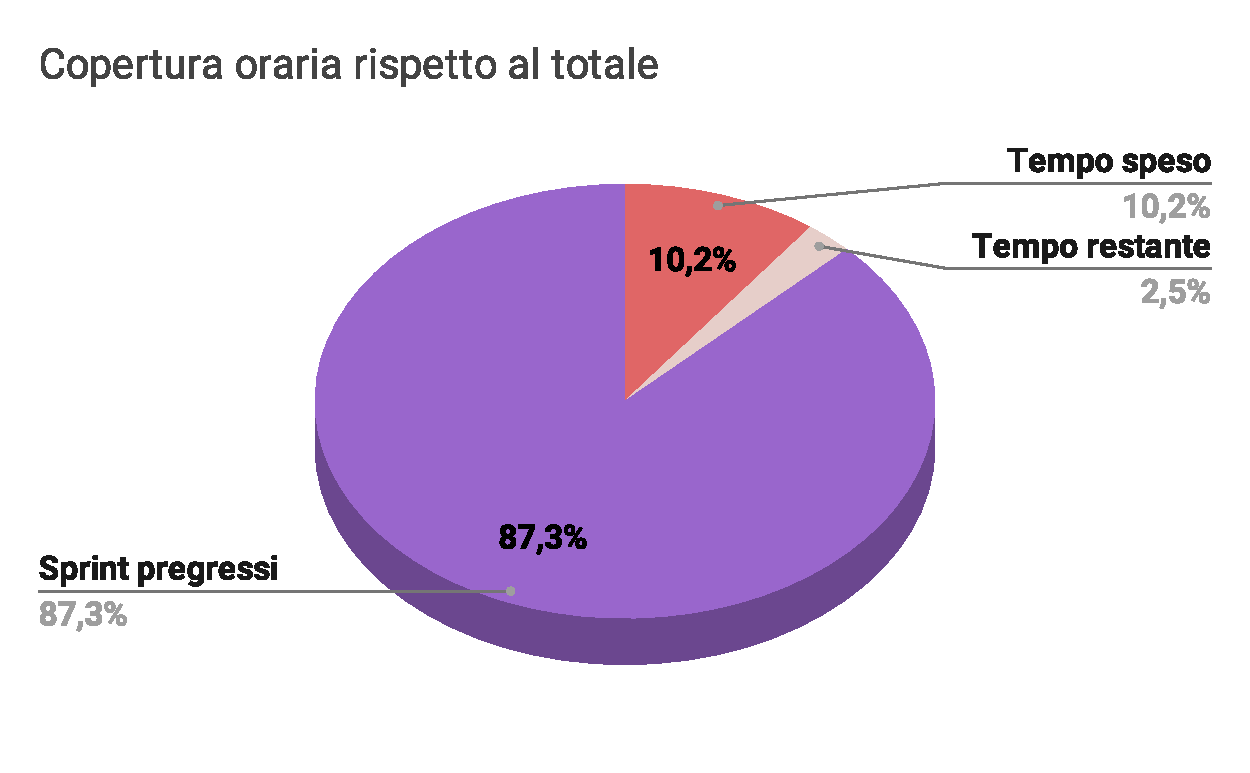
\includegraphics[width=0.90\textwidth]{assets/Consuntivo/Sprint-13/copertura_oraria.pdf}
    \caption{Sprint 13 - Areogramma del tempo speso (in ore) rispetto al totale}
  \end{figure}

  \begin{figure}[H]
    \centering
    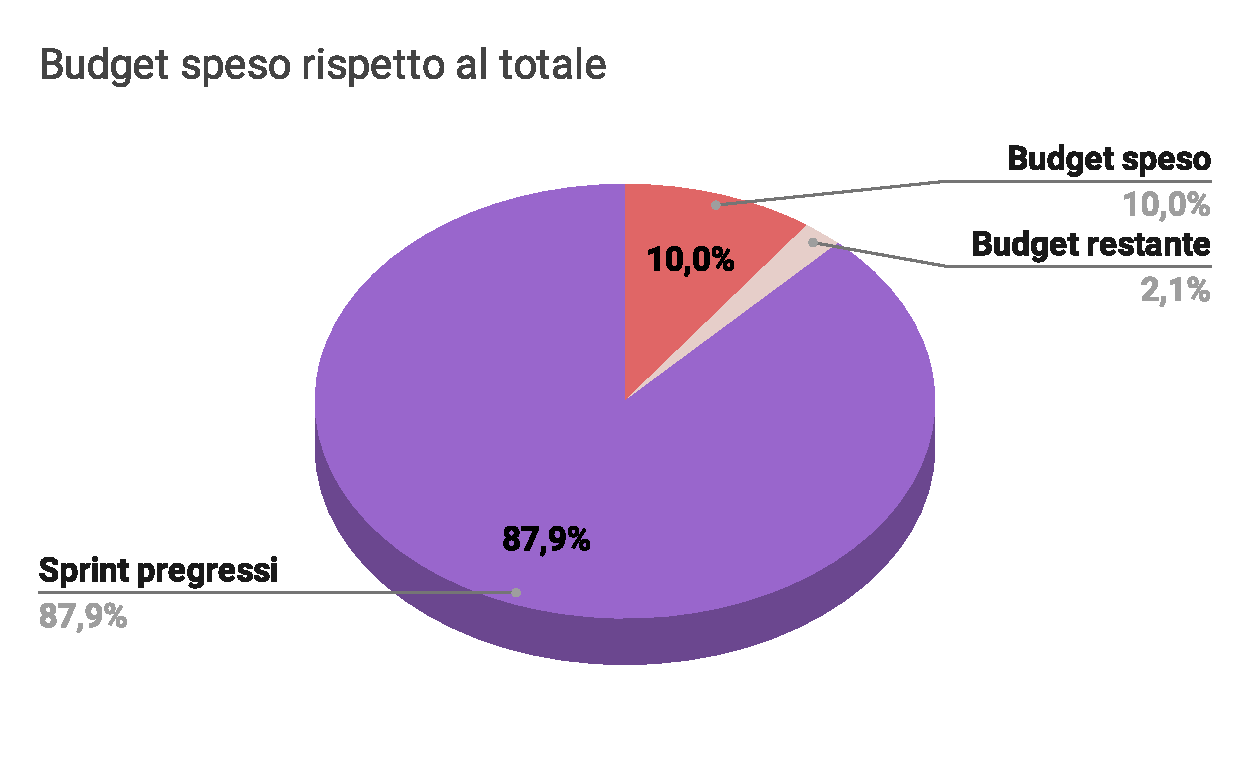
\includegraphics[width=0.90\textwidth]{assets/Consuntivo/Sprint-13/budget_speso.pdf}
    \caption{Sprint 13 - Areogramma del budget speso rispetto al totale}
  \end{figure}

  \begin{minipage}{\textwidth}
    Di seguito sono riportate le ore rimanenti per la coppia risorsa-ruolo:
    \begin{table}[H]
      \begin{tabularx}{\textwidth}{|c|*{6}{>{\centering}X|}c|}
        \hline
        \multicolumn{8}{|c|}{\textbf{Ore rimanenti per la coppia risorsa-ruolo}} \\
        \hline
        \textbf{Membro del team} & \textbf{Re} & \textbf{Am} & \textbf{An} & \textbf{Pt} & \textbf{Pr} & \textbf{Ve} & \textbf{Totale per persona} \\
        \hline
        Riccardo Cavalli & 0 & 1 & 0 & 0 & 0 & 2 & 3 \\
        \hline
        Raul Pianon & 0 & 1 & 0 & 0 & 1 & 1 & 3 \\
        \hline
        Martina Dall'Amico & 0 & 0 & 0 & 0 & 0 & 2 & 2 \\
        \hline
        Marco Cristo & 0 & 0 & 0 & 0 & 0 & 2 & 2 \\
        \hline
        Sebastiano Lewental & 1 & 0 & 0 & 0 & 0 & 1 & 2 \\
        \hline
        Mattia Zecchinato & 0 & 1 & 0 & 0 & 0 & 1 & 2 \\
        \hline
        Tommaso Stocco & 0 & 0 & 0 & 0 & 0 & 2 & 2 \\
        \hline
        \textbf{Totale ore per ruolo} & 1 & 3 & 0 & 0 & 1 & 11 & \textbf{16} \\
        \hline
      \end{tabularx}
      \caption{Sprint 13 - Ore rimanenti per la coppia risorsa-ruolo}
    \end{table}
  \end{minipage}

\subsubsection{Revisione delle attività}

Nell'arco del tredicesimo \glossario{sprint}, il team ha svolto le seguenti attività:
\begin{itemize}
  \item Revisione del documento di \AdR;
  \item Consuntivo \glossario{sprint} 12;
  \item Stesura verbali interni ed esterni;
  \item Ultimazione del cruscotto di valutazione della qualità;
  \item Implementazione di test \glossario{front-end} per migliorare la copertura del codice;
  \item Refactoring codice \glossario{back-end} e integrazione pattern Strategy;
  \item Revisione completa del codice sorgente;
  \item Aggiornamento dei grafici nel documento di \ST;
  \item Ampliamento del documento di \ST\ nelle seguenti sezioni:
  \begin{itemize}
    \item Architettura esagonale;
    \item Componenti back-end e front-end;
    \item Classi;
    \item Design pattern.
  \end{itemize}
  \item Collaudo del software;
  \item Incontro con la \glossario{Proponente} a titolo di aggiornamento sullo stato del progetto;
  \item Registrazione test di accettazione e relativo esito nel \PdQ;
  \item Integrazione Codecov-GitHub;
  \item Stesura sezioni installazione e avvio nel \MU;
  \item Revisione del documento di \ST;
  \item Rilascio del software;
  \item Organizzazione incontro con il Professor Cardin per la revisione \glossario{PB}.
\end{itemize}

\subsubsection{Retrospettiva}

\par Di seguito sono riportati i risultati del questionario di valutazione dello \glossario{sprint}:
\begin{itemize}
  \item Organizzazione dello sprint - Valutazione: 8.5;
  \item Conduzione dei meeting interni - Valutazione: 8;
  \item Impegno e partecipazione dei singoli membri - Valutazione: 7.5;
  \item Tutti i membri del team erano a conoscenza delle proprie mansioni;
  \item La numerosità delle riunioni è risultata adeguata per quasi tutti i membri del gruppo;
  \item Le riunioni sono state organizzate con il giusto preavviso;
  \item Il rapporto medio tra ore spese e ore produttive è stato inferiore a 1.5.
\end{itemize}

\vspace{0.5\baselineskip}
\par A seguire le \textbf{analisi a posteriori} del tredicesimo \glossario{sprint}:
\begin{itemize}
  \item Il team ha ricevuto l'approvazione da parte della \glossario{Proponente}, che ha confermato il raggiungimento degli obiettivi stabiliti nel capitolato;
  \item Il gruppo ha ampliato i test relativi al codice \glossario{front-end}, ottenendo una copertura complessiva superiore al 95\%;
  \item Durante le ultime fasi di codifica, il team ha testato l'integrazione tra GitHub, SonarCloud e Codecov, riscontrando un miglioramento significativo nel processo di sviluppo;
  \item Il gruppo ha integrato il pattern Strategy nel codice \glossario{back-end}, permettendo di cambiare l'algoritmo di \glossario{ricerca semantica} senza dover modificare il codice che lo utilizza;
  \item Il team ha aggiornato il tracciamento dei requisiti e il cruscotto di valutazione della qualità. I valori misurati hanno mostrato una percentuale di soddisfacimento delle metriche in linea con le aspettative.
\end{itemize}

\subsubsection{Aggiornamento pianificazione e preventivo}
\par Il team ha definito un piano d'azione per migliorare l'organizzazione e la produttività del prossimo \glossario{sprint}:
\begin{itemize}
  \item Programmare riunioni dedicate per verificare i documenti e il codice sorgente, attraverso una collaborazione stretta tra tutti i membri del gruppo.
\end{itemize}

\paragraph*{Pianificazione futura:}
\par Con il completamento dei test di sistema e di accettazione, il team ha fissato per il prossimo \glossario{sprint} la revisione \glossario{PB}. Pertanto, il gruppo si concentrerà sulla preparazione della presentazione per il colloquio con il Professor Cardin e aggiornerà la documentazione di progetto.

\paragraph*{Preventivo "a finire" (\sezione{sec:stima_temporale}):}
\par Il team intende completare il progetto entro la fine del prossimo \glossario{sprint}, rispettando sia il budget che il monte ore previsti.

\paragraph*{Gestione dei rischi (\sezione{sec:analisi_rischi}):}
\par Durante il tredicesimo \glossario{sprint}, i seguenti rischi sono stati gestiti con successo:
\begin{itemize}
  \item \textbf{RO3: Sottostima delle risorse necessarie per un'attività}: il team ha sottostimato le attività necessarie per aggiornare il documento di \ST\ e per verificare il codice e il diagramma delle classi. Tuttavia, grazie all'organizzazione di riunioni dedicate e all'uso di strumenti di collaborazione online, il gruppo è riuscito a completare le attività con il minor ritardo possibile.
\end{itemize}
